\section{Failure \& Data Distribution Mismatch}
% Slide 18
\begin{frame}{How can this approach fail?}
\centering
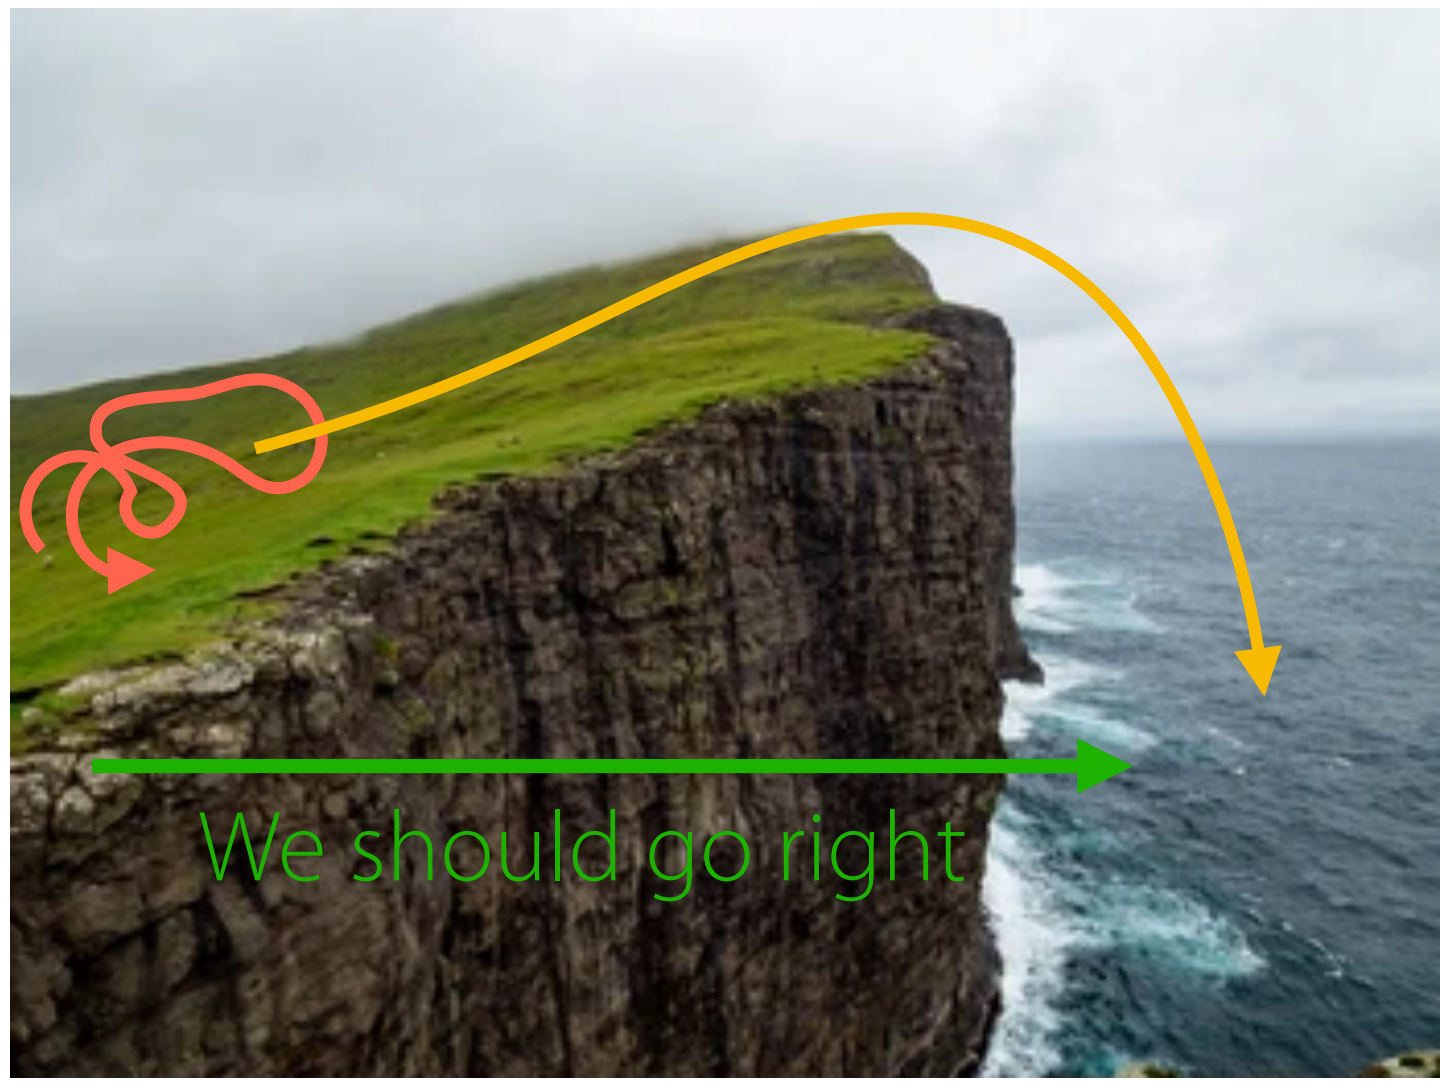
\includegraphics[width=0.42\textwidth]{images/model-based-rl/figures/cliff-fail.jpg}
\end{frame}

% Slide 19
\begin{frame}{How can this approach fail?}
\centering
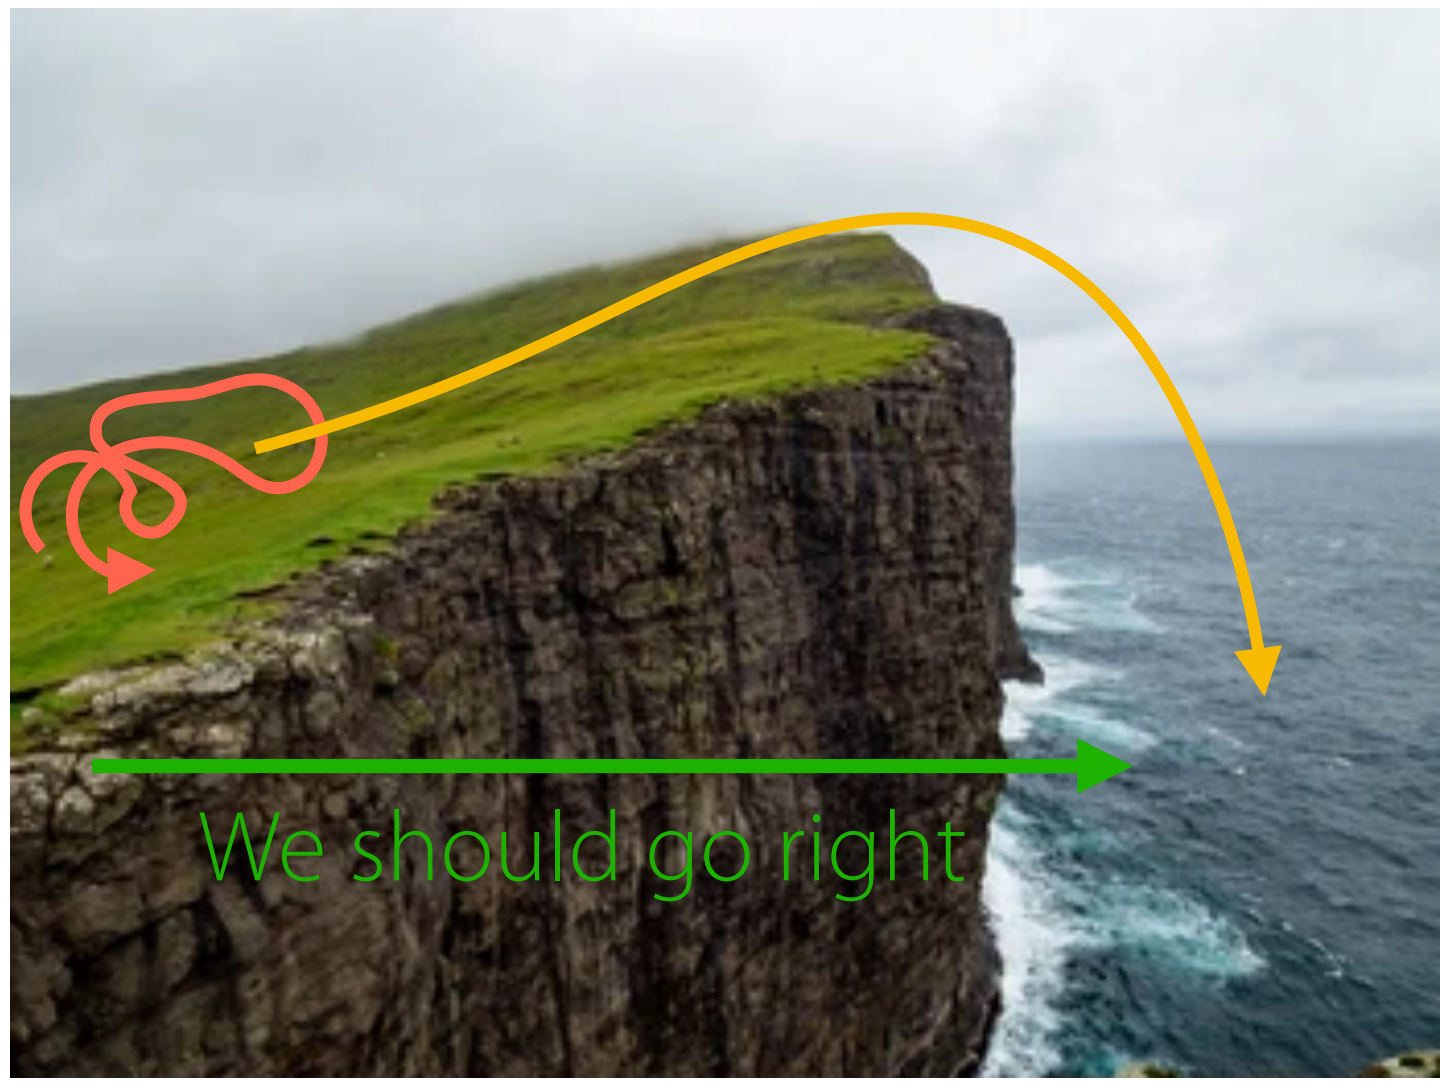
\includegraphics[width=0.36\textwidth]{images/model-based-rl/figures/cliff-fail.jpg}
\begin{itemize}
    \item In the first step, when we sample using random policy we may get
          get trajectories like the red line.
\end{itemize}
\end{frame}

% Slide 20
\begin{frame}{How can this approach fail?}
\centering
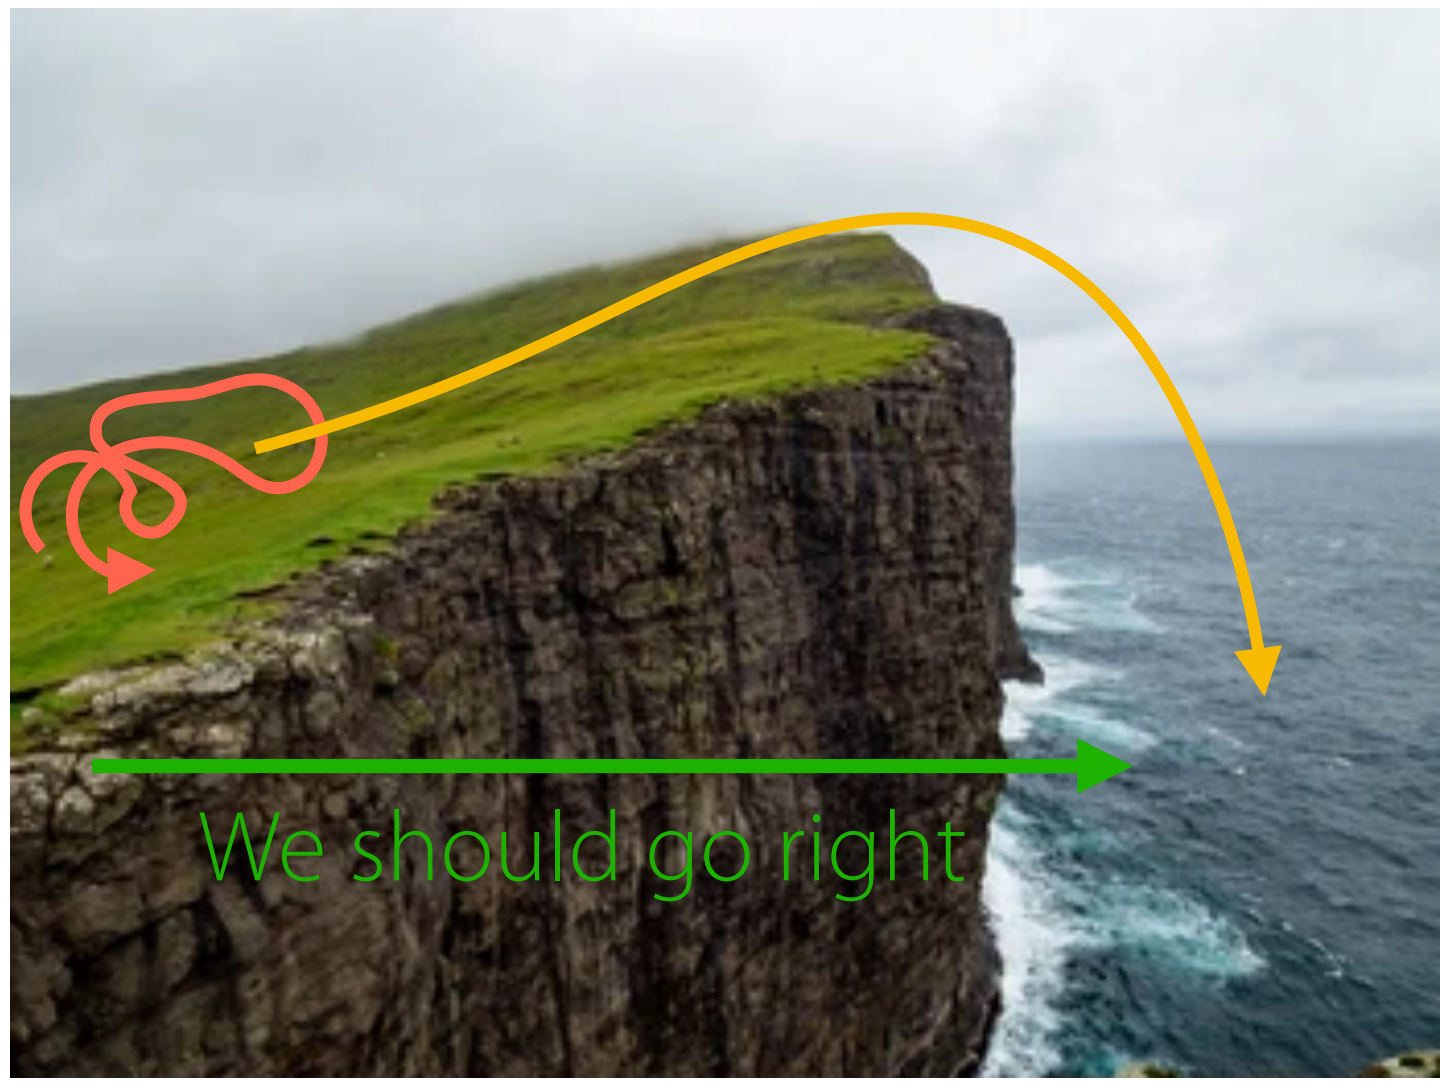
\includegraphics[width=0.36\textwidth]{images/model-based-rl/figures/cliff-fail.jpg}
\begin{itemize}
    \item In the first step, when we sample using random policy we may get
          get trajectories like the red line.
    \item The agent may learn that going right means that we can go higher!
\end{itemize}
\end{frame}

% Slide 21
\begin{frame}{How can this approach fail?}
\centering
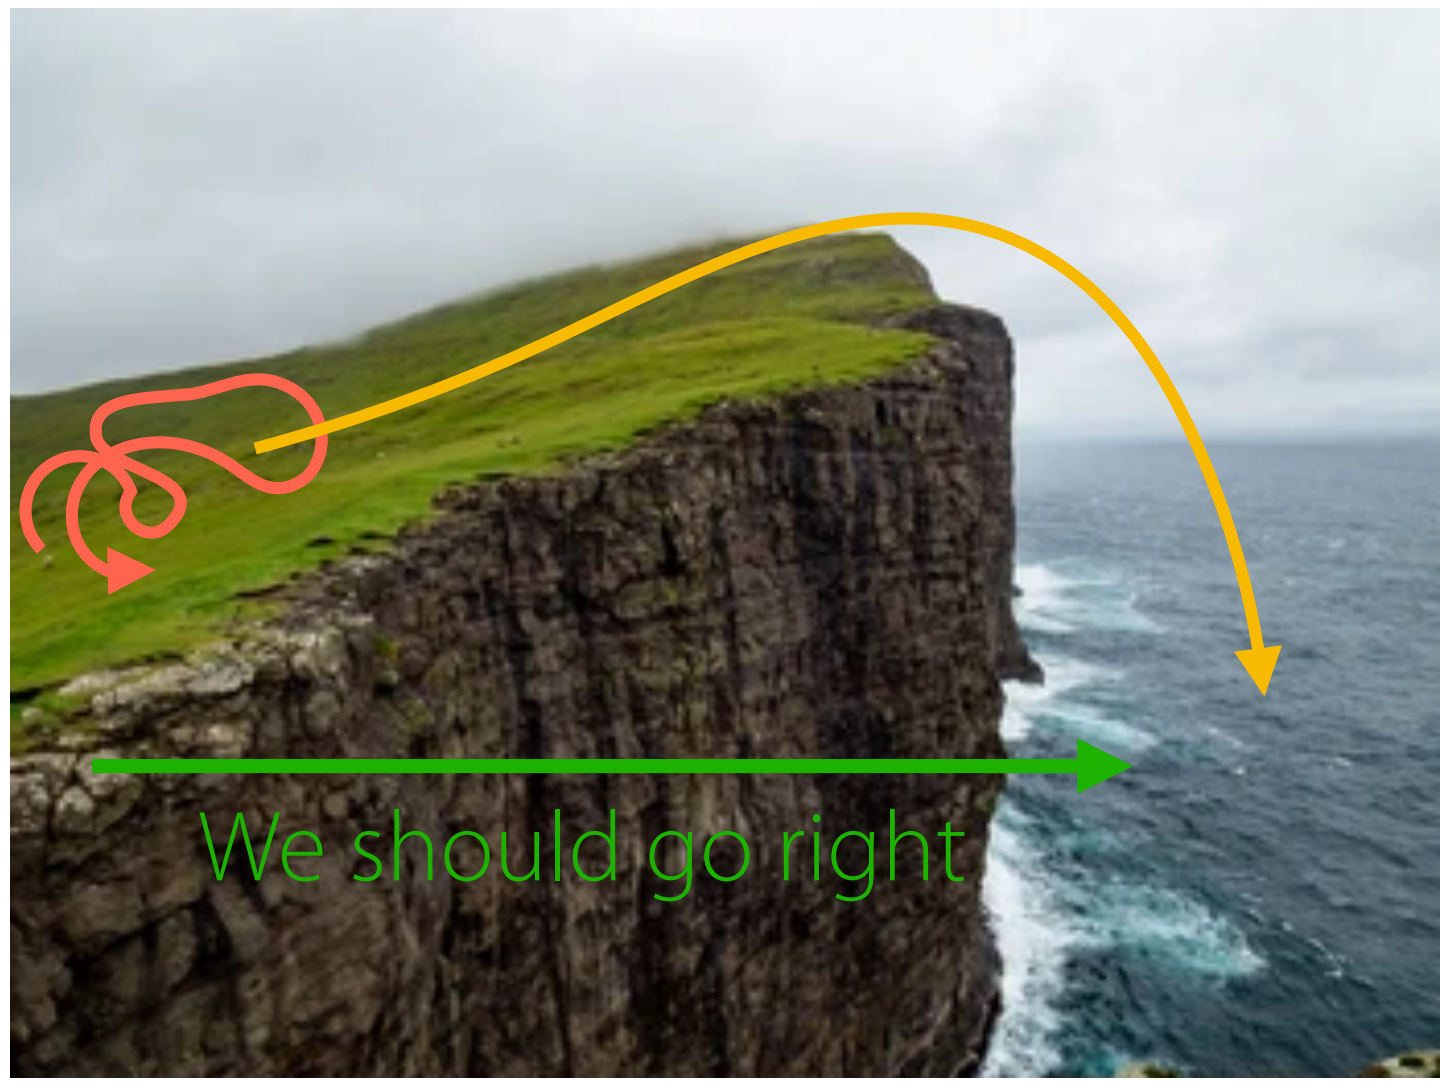
\includegraphics[width=0.36\textwidth]{images/model-based-rl/figures/cliff-fail.jpg}
\begin{itemize}
    \item In the first step, when we sample using random policy we may get
          get trajectories like the red line.
    \item The agent may learn that going right means that we can go higher!
    \item Thus, it will learn an incomplete policy and fall at the top.
\end{itemize}
\end{frame}

% Slide 22
\begin{frame}{How can this approach fail?}
\centering
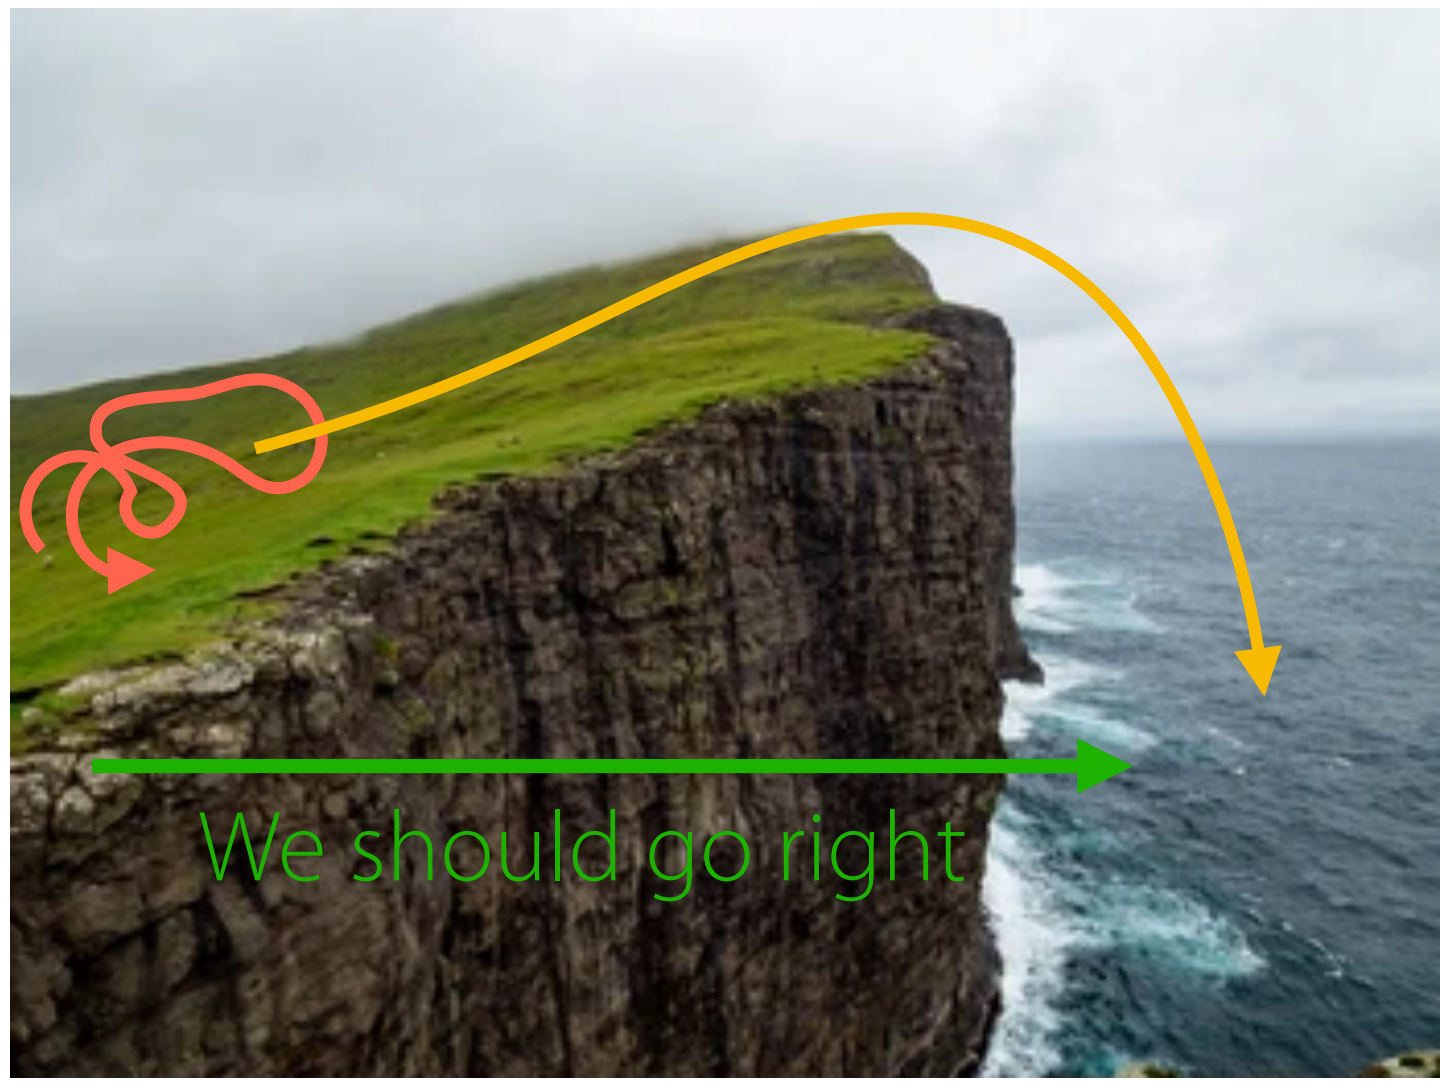
\includegraphics[width=0.36\textwidth]{images/model-based-rl/figures/cliff-fail.jpg}
\begin{itemize}
    \item In the first step, when we sample using random policy we may get
          get trajectories like the red line.
    \item The agent may learn that going right means that we can go higher!
    \item Thus, it will learn an incomplete policy and fall at the top.
    \item The model was only trained where the \emph{random} policy went, but the
          planner now wants to go somewhere the model has never seen
\end{itemize}
\end{frame}

% Define the mismatch precisely.
\begin{frame}{Why? A Distribution Mismatch}
\begin{itemize}
    \item Write $p_\pi(s)$ for \textbf{how often the agent visits state $s$ when
          it follows policy $\pi$} (its distribution over states)
\end{itemize}
\end{frame}

\begin{frame}{Why? A Distribution Mismatch}
\begin{itemize}
    \item Write $p_\pi(s)$ for \textbf{how often the agent visits state $s$ when
          it follows policy $\pi$} (its distribution over states)
    \item $\pi_0$ (the policy that \textbf{collected the data}, e.g.\ the random
          policy) spends its time near the \emph{bottom} of the cliff
    \item $\pi_f$ (the \textbf{final} policy after planning) wants to climb to the
          \emph{top}
\end{itemize}
\end{frame}

\begin{frame}{Why? A Distribution Mismatch}
\begin{itemize}
    \item Write $p_\pi(s)$ for \textbf{how often the agent visits state $s$ when
          it follows policy $\pi$} (its distribution over states)
    \item $\pi_0$ (the policy that \textbf{collected the data}, e.g.\ the random
          policy) spends its time near the \emph{bottom} of the cliff
    \item $\pi_f$ (the \textbf{final} policy after planning) wants to climb to the
          \emph{top}
    \item So the states shift from the \emph{data} distribution to the
          \emph{learned-policy} distribution:
    \[ \underbrace{p_{\pi_0}(s)}_{\text{where we trained}} \;\neq\;
       \underbrace{p_{\pi_f}(s)}_{\text{where we now act}} \]
    \item The model is accurate on $p_{\pi_0}$ but gets asked to predict on
          $p_{\pi_f}$, exactly where it never saw data
    \item Remember this picture; we return to it for \emph{offline RL}
\end{itemize}
\end{frame}
